\documentclass{curriculum_vitae}

\begin{document}
% \photo[64pt][0.4pt]{picture} 

    \makecvtitle
    % 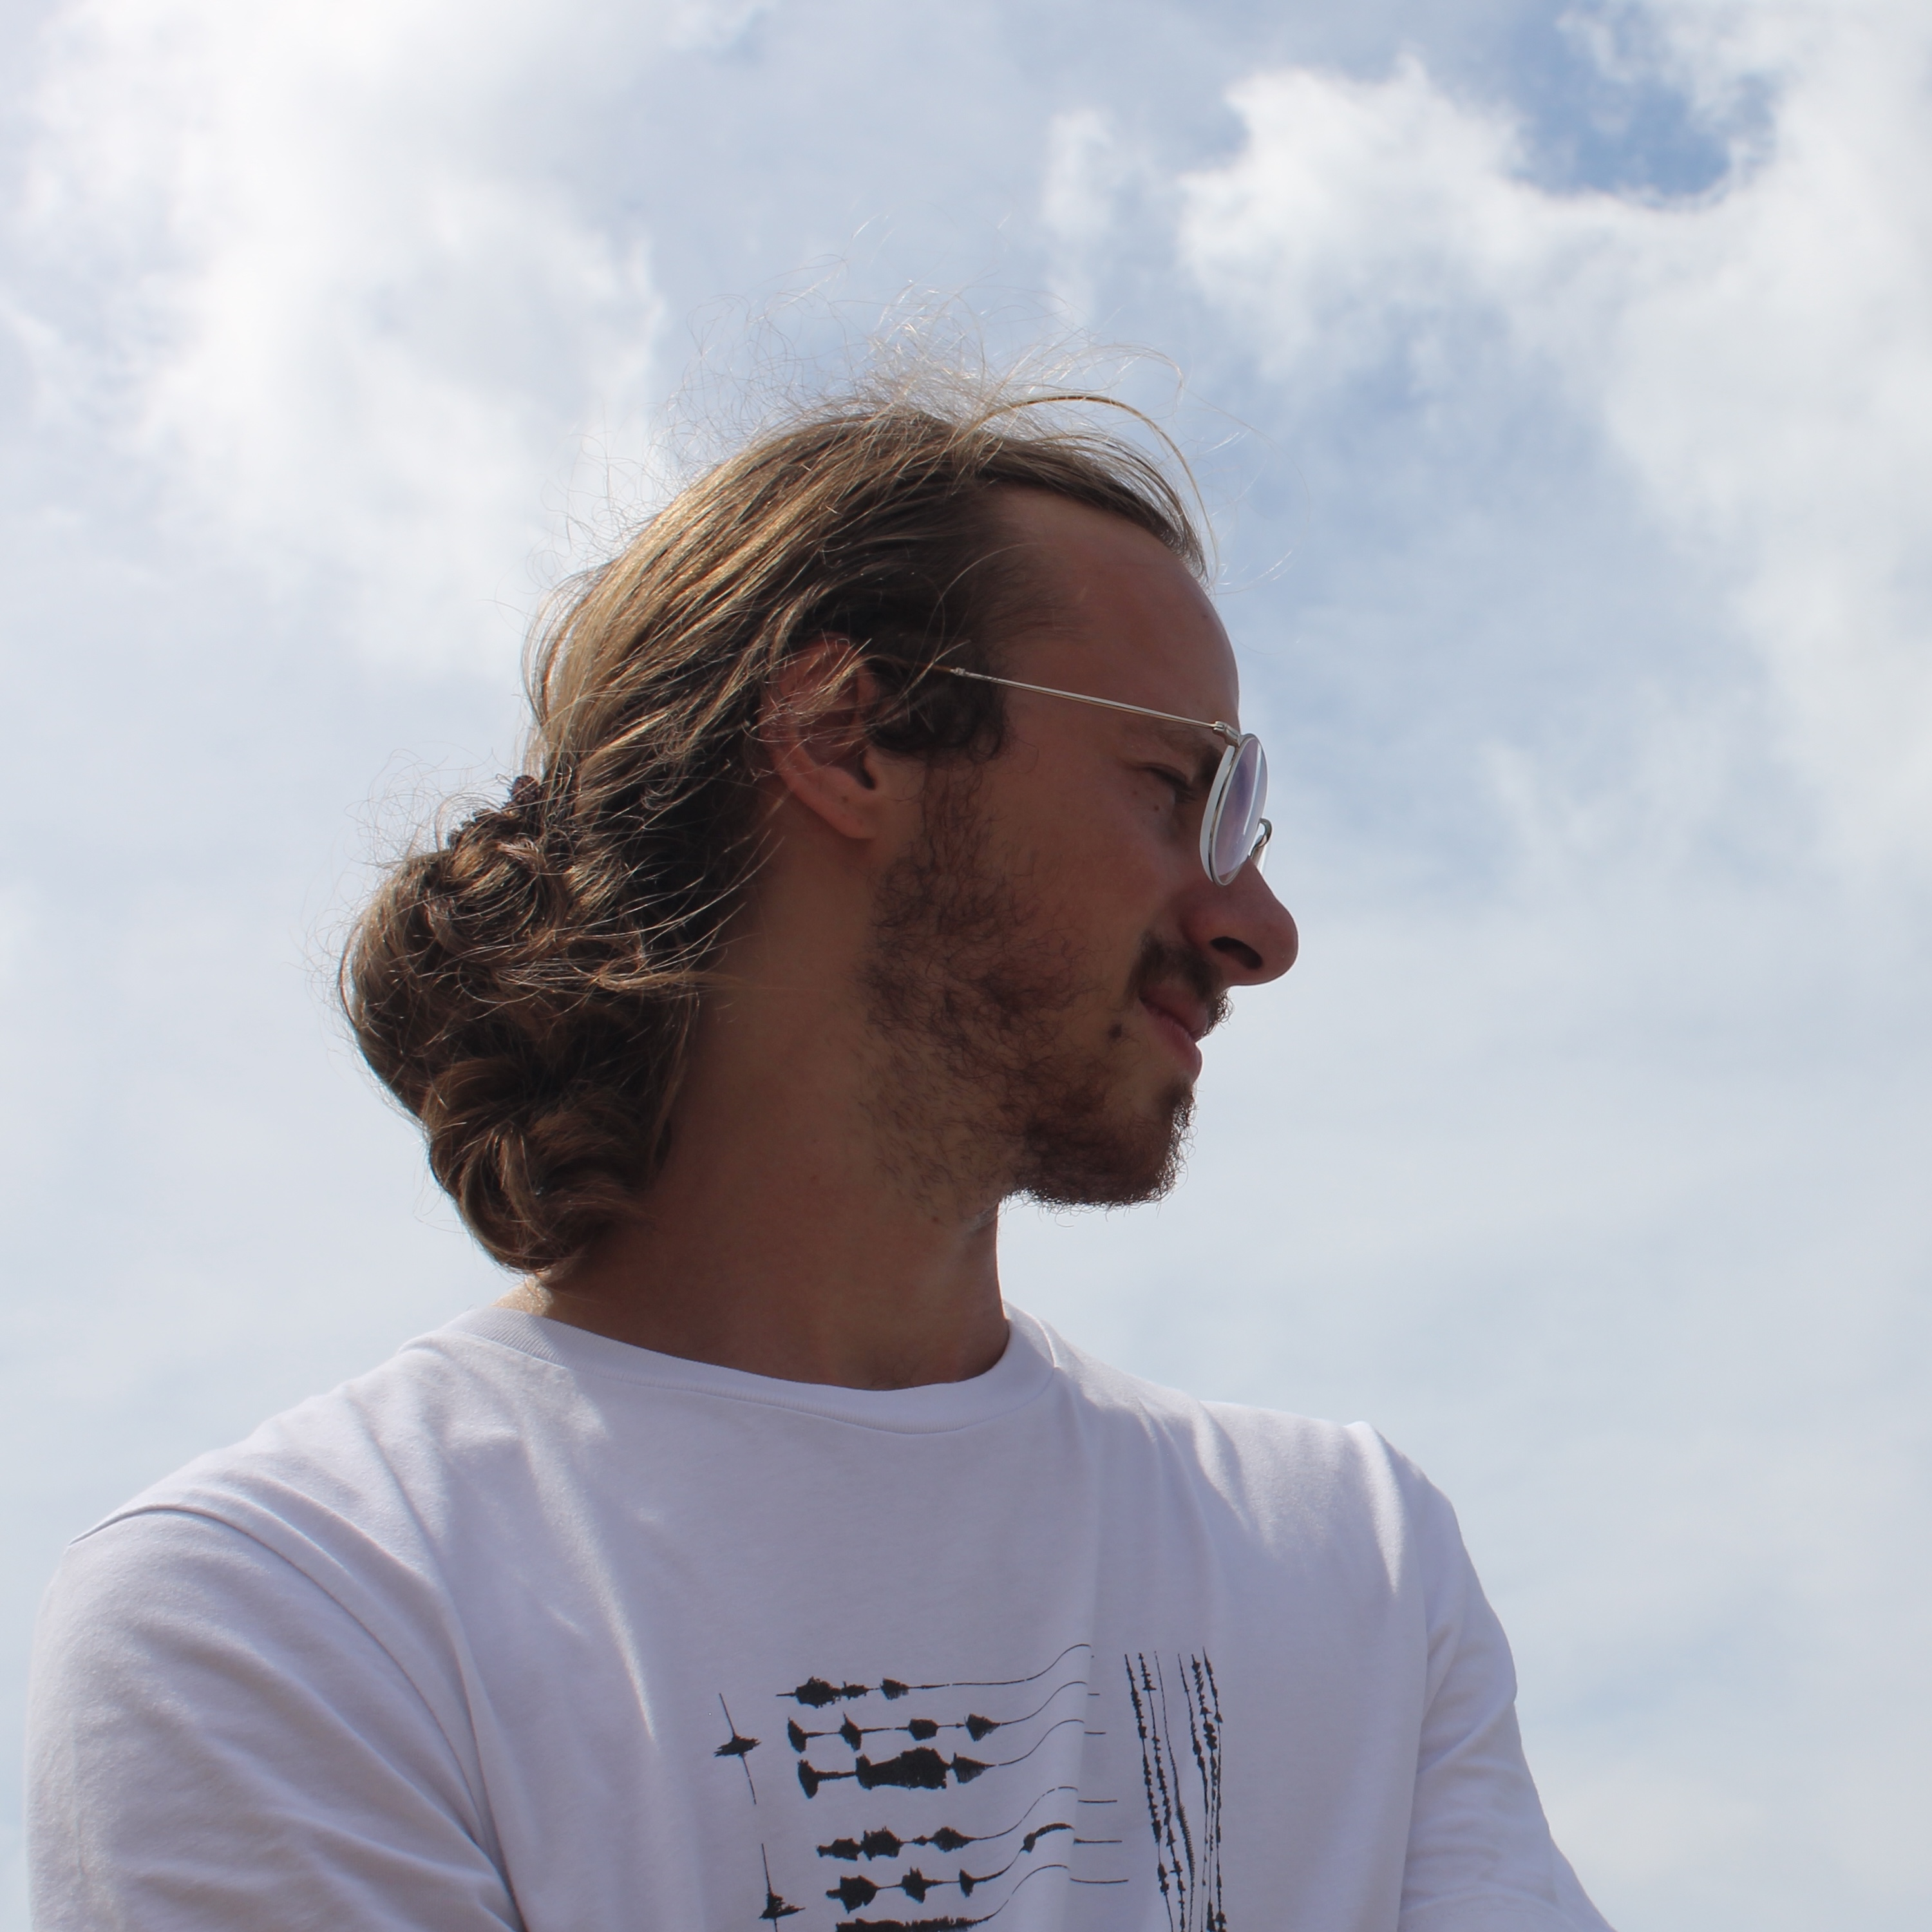
\includegraphics[width=0.8\linewidth]{./picture.jpg}
    
    \section{Personal Details}
        \cvitem{Name}{Mader, Vincent Christian}
        \cvitem{City of Birth}{Ulm-Söflingen, Germany}
        \cvitem{Date of Birth}{July 11th, 1998}
        \cvitem{Nationality}{German}
    % \section{Pers\"onliche Daten}
    %     \cvitem{Name}{Mader, Vincent Christian}
    %     \cvitem{Geburtsdatum}{11. Juli 1998}
    %     \cvitem{Geburtsort}{Ulm, Deutschland}
    %     \cvitem{Nationalit\"at}{Deutsch}
    
    \section{Education}
        % \cventry{2004--2008}{J\"org-Syrlin-Grundschule}{}{Ulm}{}{}
        \cventry{2008 -- 2016}{Hans-und-Sophie-Scholl-Gymnasium}{Abitur}{Ulm}{}{} 
        \cventry{2016 -- 2020}{Ruprecht Karl University of Heidelberg}{Bachelor of
        Science in Physics}{Heidelberg}{}{}
        \cventry{2020 -- 2024}{Ruprecht Karl University of Heidelberg}{Master of
        Science in Physics}{Heidelberg}{}{} 
    % \section{Ausbildung}
        % \cventry{2004--2008}{J\"org-Syrlin-Grundschule}{}{Ulm}{}{}
        % \cventry{2008--2016}{Hans-und-Sophie-Scholl-Gymnasium}{}{Ulm}{}{} 
        % \cventry{2016--2020}{Ruprecht-Karls-Universit\"at}{Bachelor-Studiengang im Fach Physik}{Heidelberg}{}{Bachelor-Arbeit am Heidelberger Max-Planck-Institut f\"ur Astronomie}
        % \cventry{seit 2020}{Ruprecht-Karls-Universit\"at}{Master-Studiengang im Fach Physik}{Heidelberg}{}{} 
   
    \section{Experience}
        \cventry{since 2015}{Physics \& Mathematics Tutor for High School
        Students}{}{}{}{}
        \cventry{2019}{Project Internship: Simulation of Accreting Planets}{Max Planck Institute for
        Astronomy}{Heidelberg}{}{}
        \cventry{Apr 2020 -- Jul 2020}{Academic Tutor for Physics Experiments}{Ruprecht Karl University of Heidelberg}{Heidelberg}{}{}
        \cventry{Feb 2021 -- Mar 2021}{Academic Tutor for Physics Experiments}{Ruprecht Karl University of Heidelberg}{Heidelberg}{}{}
        \cventry{Oct 2022 -- Jan 2023}{Academic Tutor for Physics Experiments}{Ruprecht Karl University of Heidelberg}{Heidelberg}{}{}
        \cventry{2022 -- 2023}{Project Internship: Utilizing Monte Carlo Sampling for the Numerical Integration of the Smoluchowski Coagulation Equation}{Institute for Theoretical Astrophysics}{Heidelberg}{}{}
        \cventry{2022 -- 2024}{Part-Time Staff in the Gastronomy Sector}{gastroevents GmbH \& Co.
        KG}{Ulm}{}{}

    % \section{Sprachkenntnisse}
    %     \cvitemwithcomment{Deutsch}{Muttersprache}{}
    %     \cvitemwithcomment{Englisch}{Fließend in Wort und Schrift}{}
    %     \cvitemwithcomment{Franz\"osisch}{? Grundkenntnisse in Wort und Schrift}{}
    %     \cvitemwithcomment{Italienisch}{? Grundkenntnisse}{}
    %     \cvitemwithcomment{Latein}{kleines Latinum}{}
        % intermediate Latin certificate
    \section{Languages}
        \cvitemwithcomment{German}{Native Language}{}
        \cvitemwithcomment{English}{Full Working Proficiency (Bilingual Education at High School)}{}
        \cvitemwithcomment{Italian}{Elementary Proficiency (A2 Certificate)}{}
        \cvitemwithcomment{French}{Elementary Proficiency}{}
        \cvitemwithcomment{Latin}{Latinum}{}
    
    \section{Skills}
        \cvitem{General}{%
            Physics, Mathematics, Computational Physics, 
            Numerical Simulation, Data Analysis, Data Visualization,
            Software Development, Web Development, App Development
        }{}
        % \cvitemwithcomment{Software}{Web/App Development, Computational Physics}{}{}
        \cvitem{Computer Languages}{% 
            Python, Rust, JavaScript, Shell Scripting, Swift, Dart, HTML, CSS, LaTeX, 
            (\& a little bit of C and Java)
        }{}
        \cvitemwithcomment{Software Tools}{%
            Linux/UNIX, Git, Docker, SSH, Vim, Emacs}{} 
        \cvitem{Social}{Team Coordination, Team Leadership, Tutoring, Children}{}
        % \cvitemwithcomment{basic}{C/C++, slurm}{}
        % \cvitemwithcomment{python}{advanced (numpy, matplotlib, scipy, torch, ...)}{}
        % \cvitemwithcomment{UNIX shell}{advanced}{}
        % \cvitemwithcomment{LaTeX}{advanced}{}
        % \cvitemwithcomment{JavaScript}{intermediate}{}
        % \cvitemwithcomment{HTML/CSS}{intermediate}{}
        % \cvitemwithcomment{git}{intermediate}{}
        % \cvitemwithcomment{C/C++}{basics}{}
        % \cvitemwithcomment{various}{git, LaTeX, UNIX shell}{}
        %\cvitemwithcomment{vi/vim/neovim}{gut}{}
        % \cvitemwithcomment{slurm}{basics}{}
        %\cvitemwithcomment{Java}{Grundkenntnisse}{}
        
    \section{Volunteering}
        \cventry{2013 -- 2015}{Children's Supervisor}{Ruhetal Ulm (two-week summer camp)}{Ulm}{}{}
        \cventry{2022 -- 2023}{Cash Auditor (Kassenprüfer)}{DPSG Bezirk Ostalb}{}{}{}
        \cventry{2022 -- 2023}{Scout Group Leader (Gruppenleiter)}{DPSG Heidelberg-Kirchheim}{Heidelberg}{}{}
        % \cventry{2015}{internship at Sonnenheim Ulm kindergarden}{}{}{}{}
        \cventry{2019 -- present}{Scout Group Leader (Gruppenleiter)}{DPSG Ulm-Söflingen}{Ulm}{}{}
        \cventry{2022 -- present}{Chair of Association (Vereinsvorsitzender)}{DPSG
        Ulm-Söflingen}{Ulm}{}{}
        \cventry{2024 -- present}{Election Committee Member (Wahlausschuss)}{DPSG Bezirk Ostalb}{}{}{}
        %\cvlistitem{Item 1}
        %\cvlistdoubleitem{Item 2}{Item 3}

\end{document}
